% !TeX spellcheck = en_US
\documentclass[11pt,a4paper]{article}
\usepackage[utf8]{inputenc}
\usepackage{amsmath}
\usepackage{amsfonts}
\usepackage{amssymb}
\usepackage{graphicx}
\usepackage{mathtools}
\usepackage[hidelinks]{hyperref}  % most people dont know of this :3

\usepackage{subfig}
\usepackage[margin=0.7in]{geometry}

% \usepackage[backend=bibtex,style=verbose-ibid]{biblatex}
% \addbibresource{citations.bib}

\usepackage{listings}
\usepackage{color}
\definecolor{dkgreen}{rgb}{0,0.6,0}
\definecolor{gray}{rgb}{0.5,0.5,0.5}
\definecolor{mauve}{rgb}{0.58,0,0.82}

\lstset{frame=tb,
  language=Python,
  aboveskip=3mm,
  belowskip=3mm,
  showstringspaces=false,
  columns=flexible,
  basicstyle={\small\ttfamily},
  numbers=none,
  numberstyle=\tiny\color{gray},
  keywordstyle=\color{blue},
  commentstyle=\color{dkgreen},
  stringstyle=\color{mauve},
  breaklines=true,
  breakatwhitespace=true,
  tabsize=3
}


\newcommand{\inv}{^{\raisebox{.2em}{$\scriptscriptstyle-1$}}}
\newcommand{\qed}{\hfill $\blacksquare$}

\newcommand{\integers}{\mathbb{Z}}
\newcommand{\rationals}{\mathbb{Q}}
\newcommand{\reals}{\mathbb{R}}
\newcommand{\complexes}{\mathbb{C}}
\newcommand{\field}{\mathbb{F}}

\author{Jacob Bruner}
\title{Bivariate Statistics Exploration}
\date{\today}

\begin{document}
\maketitle
% \tableofcontents

% \pagebreak

\iffalse
############
heres an example of a code block
\begin{lstlisting}
        def intervalValues(z, n):
            return output # return the sequence of values
\end{lstlisting}

heres an example of an image
\begin{figure}[h]
\begin{center}
\includegraphics[scale=.37]{onefifteen} 
\caption{Sequences Generated by n = 1-15 on Argand Diagram}
\end{center}
\end{figure}
############
\fi

\section{Introduction}

In the real-world, statistics are often employed as objective measures of data. Because of this, we often draw important, life-changing decisions on their basis alone. For instance, pharmacists employ statistics when researching new treatments for disease, or economists might draw on statistics to understand trends in consumer spending. Luckily for us, statistics often \textit{are} helpful and insightful in disseminating patterns in data. But, again, it is all too easy to forget their short-comings.

In 1973, British mathematician Francis Anscombe formulated four datasets, each with 11 points, in order to demonstrate the pitfalls of many common statistical measures. In this paper, I will explore the ways in which these statistical measures can be misleading in interpreting the significance of, trends in, or validity of data using Anscombe's 'quartet' of points to highlight their oversimplification.

\section{The Statistical Mean}
\subsection{Computation}
The mean is a commonly used measure of center for a given statistic. To calculate the mean, we can use the following formula: for a given indexed set of values, the mean is written:
\[
\bar{x} = \frac{1}{N} \sum_{i = 1}^{N} x_i
\]
Where N is the length of the data set. In other words, the mean is the sum of each value divided by the number of values for a given parameter. \\


Calculating these values for each dataset we obtain:

\begin{figure}[ht]
\centering
\begin{tabular}{|l|cc|cc|cc|cc|}
\hline
\textbf{Data set}         & \multicolumn{2}{c|}{\textbf{I}}              & \multicolumn{2}{c|}{\textbf{II}}             & \multicolumn{2}{c|}{\textbf{III}}            & \multicolumn{2}{c|}{\textbf{IV}}             \\ \hline
\textbf{Parameter} & \multicolumn{1}{c|}{\textit{x}} & \textit{y} & \multicolumn{1}{c|}{\textit{x}} & \textit{y} & \multicolumn{1}{c|}{\textit{x}} & \textit{y} & \multicolumn{1}{c|}{\textit{x}} & \textit{y} \\ \hline
\textbf{Mean}     & \multicolumn{1}{c|}{9.0}        & 7.5        & \multicolumn{1}{c|}{9.0}        & 7.5        & \multicolumn{1}{c|}{9.0}        & 7.5        & \multicolumn{1}{c|}{9.0}        & 7.5        \\ \hline
\end{tabular}
\caption{Computed Means of Dataset I-IV}
\end{figure}

\subsection{Interpretation}

After computing the mean for each, it's clear that the means for each $x, y$ of the respective datasets are equal. Without any other prior knowledge, one might infer that these datasets have a similar center, save variation or spread. This is because the mean doesn't provide information about the variation or spread of the data. Despite this, however, one might assume it to be a reasonable assumption that these datasets and parameters might be highly similar, especially because they match in two variables.

\section{Exploring Other Statistical Measures}
\subsection{Computation}

In addition to computing the mean, there are a number of other tools that provide insight into the properties of a dataset. For instance, the \textbf{\textit{variance}} ($\sigma^2$) and \textbf{\textit{standard deviation}} ($\sigma$) convey a measure of the 'spread' or variation in a dataset. Similarly, \textbf{\textit{'Peterson's Correlation Coefficient'}} ($r$) often denoted with its square, $r^2$, is measure of the \textit{linear} coorelation of two parameters. (Unsquared) values of $r$ range from -1 to 1, with numbers farther from zero denoting stronger coorelation. A closely related notion is the \textbf{\textit{covariance}}, which measures the linear coorelation, but with a magnitude not necessarily between $(-1, 1)$. These measures are related like so: $r = \frac{cov(x, y)}{\sigma_x \sigma_y}$ where $\sigma$ denotes the standard deviation.

\begin{figure}[]
\centering
\begin{tabular}{l|c|c|c|c|c|c|c|c|}
\cline{2-9}
                                     & \textbf{$\bar{x}$} & \textbf{$\bar{y}$} & \textbf{$\sigma_x^2$} & \textbf{$\sigma_y^2$} & \textbf{$\sigma_x$} & \textbf{$\sigma_y$} & \textbf{$r^2$} & \textbf{$cov(x, y)$} \\ \hline
\multicolumn{1}{|l|}{\textbf{set 1}} & 9.0                & 7.5              & 11.0                & 4.13                & 3.32                  & 2.03                  & 0.67           & 5.5                  \\ \hline
\multicolumn{1}{|l|}{\textbf{set 2}} & 9.0                & 7.5              & 11.0                & 4.13                & 3.32                  & 2.03                  & 0.67           & 5.5                  \\ \hline
\multicolumn{1}{|l|}{\textbf{set 3}} & 9.0                & 7.5              & 11.0                & 4.12                & 3.32                  & 2.03                  & 0.67           & 5.5                  \\ \hline
\multicolumn{1}{|l|}{\textbf{set 4}} & 9.0                & 7.5              & 11.0                & 4.12                & 3.32                  & 2.03                  & 0.67           & 5.5                  \\ \hline
\end{tabular}
\caption{Comparison of different Statistical Measures of Datasets I-IV}
\end{figure}

\subsection{Plotting Data}

Using the python packages \texttt{matplotlib}, \texttt{scipy}, \texttt{numpy} and \texttt{pandas}, we can plot each dataset (as a dataframe contained in the array \texttt{dfs}). A linear regression is fit to the data using the \texttt{np.polyfit()} method with an exponent of 1, and the Pearson's coefficent is calculated using the \texttt{stats.pearsonr()} method. This is accomplished like so:

\begin{lstlisting}
for i in range(4):
  dfs[i].plot.scatter(x='x', y='y') 
  reg = np.polyfit(dfs[i]['x'], dfs[i]['y'], 1)
  rval = stats.pearsonr(dfs[i]['x'], dfs[i]['y'])[0]
  plt.plot(dfs[i]['x'], np.polyval(reg, dfs[i]['x']), 'r', label='y={:.2f}x+{:.2f}\n r^2 = {:.2f}'.format(reg[0], reg[1], rval**2))
  plt.xlabel('x')
  plt.ylabel('y')
  plt.legend()
  plt.savefig('dataset{}.png'.format(i+1))
\end{lstlisting}

In so doing, we get the following interesting results (Figure~\ref{fig:plots}):

\begin{figure}[ht]
\centering
\subfloat[Dataset I]{\label{fig:I}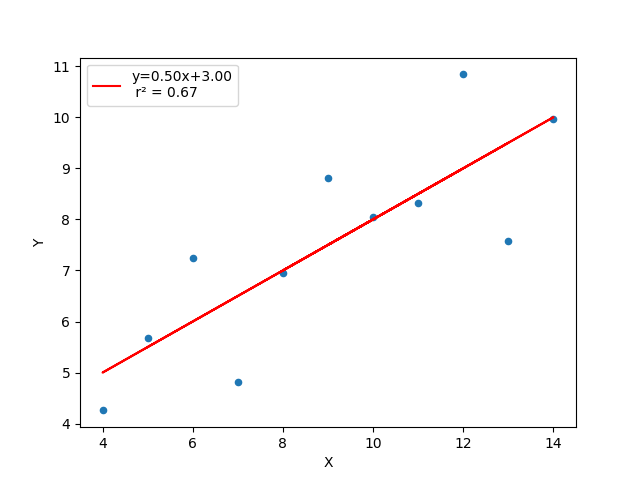
\includegraphics[width=0.45\linewidth]{dataset-1.png}}\qquad
\subfloat[Dataset II]{\label{fig:II}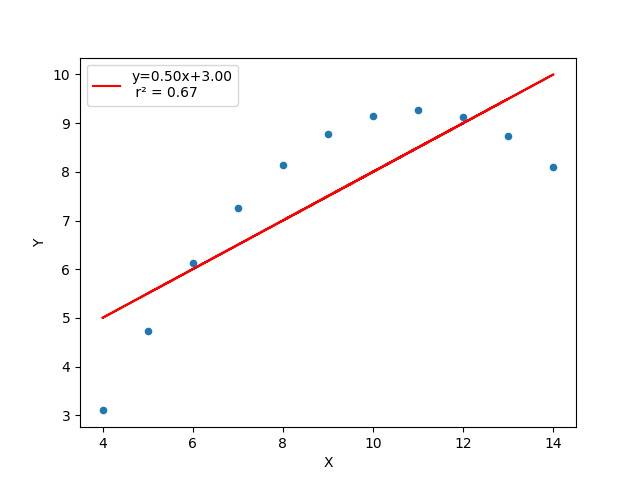
\includegraphics[width=0.45\linewidth]{dataset-2.png}}\\
\subfloat[Dataset III]{\label{fig:III}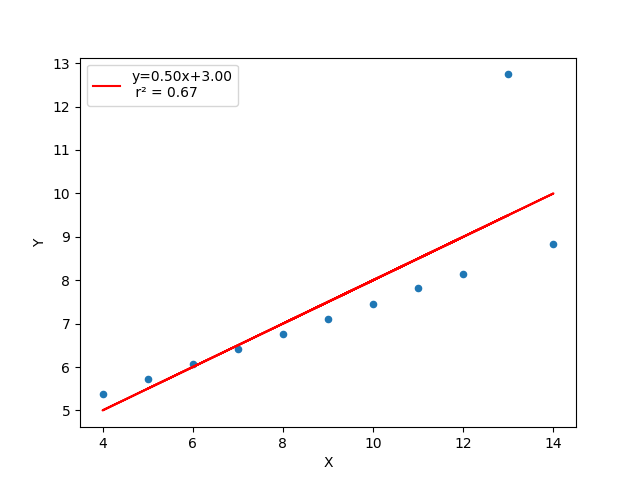
\includegraphics[width=0.45\textwidth]{dataset-3.png}}\qquad%
\subfloat[Dataset IV]{\label{fig:IV}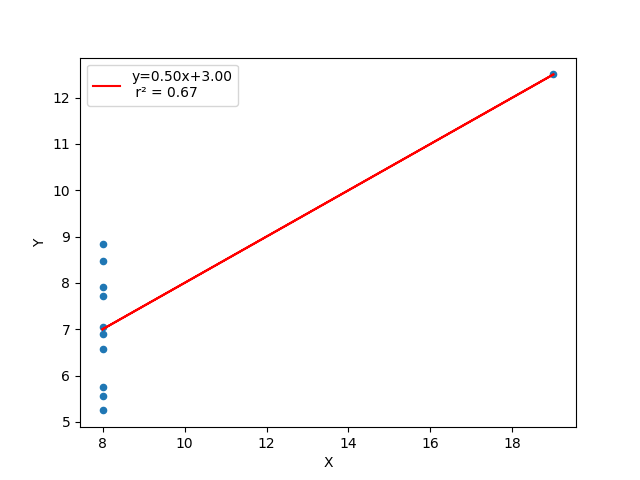
\includegraphics[width=0.45\textwidth]{dataset-4.png}}%
\caption{Plot of Datasets I-IV — X against Y with Lin. Reg.}
\label{fig:plots}
\end{figure}

\subsection{Interpretation}

Upon examination of the computed statistical measures (std, variance, cov, etc.), the naive conclusion would be that each dataset contains extremely similar data and that similar conclusions could be drawn from each. For instance, the $r^2$ value for each, $0.67$, indicates that there is a weak-to-moderate, positive correlation between the variables, and might imply that linear fits to each dataset would have a similar degree of inaccuracy. However, this notion is \textit{categorically refuted} on even a cursory glance at the graphs. In Figure~\ref{fig:plots}, we see that each dataset is very distinct in its scatterplot pattern. In Figure~\ref{fig:I}, its clear that the linear fit to the data indicates weak-moderate, positive correlation, with a healthy amount of deviation from the trendline. This graph's, the most straightforward of the four, statistical measures indicate helpful information about the data. For instance, the $r^2$ value of $0.67$ reinforces the weak, positive spread outlined above. Similarly, the covariance of $5.5$ and the variance $\sigma_x^2 = 11.0,\ \sigma_y^2 = 4.13$ reinforce the visual intuition of this dataset having a healthy amount of spread from the means $\bar{x}, \bar{y}$. 
As we transition to Figure~\ref{fig:II}, we see a markedly different trend in the data. Visually, the scatterplot indicates an quadratic trend in $x$, indicating that the $y$ values may vary as the negative square of $x$. Despite this, our linear trendlines (from a least squares regression) provides a line of 'best fit' equal to Figure~\ref{fig:I}. Additionally, the other statistical measures of dataset II are exactly equivalent to that of dataset I, despite the visual interpretation being different. For instance, one might interpret the $r^2$ value in Figure~\ref{fig:I} as indicating the moderate (seemingly random) variation from the trendline, whereas in Figure~\ref{fig:II}, we see the datapoints follow exactly the (not random) curve of a quadratic, despite still having the same $r^2$. If one were to perform a polynomial regression (perhaps taking the logarithm to linearize the polynomial exponent, then performing a least squares regression), the resulting trendcurve would likely be an extremely close fit to the data---a fact not illustrated by these statistical measures. 
In Figure~\ref{fig:III}, we see a different outcome where, despite displaying a very linear trend, the computed statistics and trendline are greatly affected by a single outlier. Because of this, we see the trendline having the incorrect slope to match the (linear) trend in the rest of the data. Despite this outlier not being indicated in the computed statistical measures, viewing the graph demonstrates the highly linear relationship between x and y, which would be easily illustrated by removing the outlier or otherwise explaining it in the methodology. This fact highights the differnce between dataset III and dataset I, where, despite having the same statistical measures, Figure~\ref{fig:I} displays almost uniformly random deviation from the line of best fit compared to Figure~\ref{fig:III} which has a nicely behaved deviation given by the intersection of another trendline if the sole outlier were to be removed.
In Figure~\ref{fig:IV}, we see how the 

\section{Exploring Other Techniques}

\begin{figure}[ht]
\centering
\subfloat[Dataset I]{\label{fig:rI}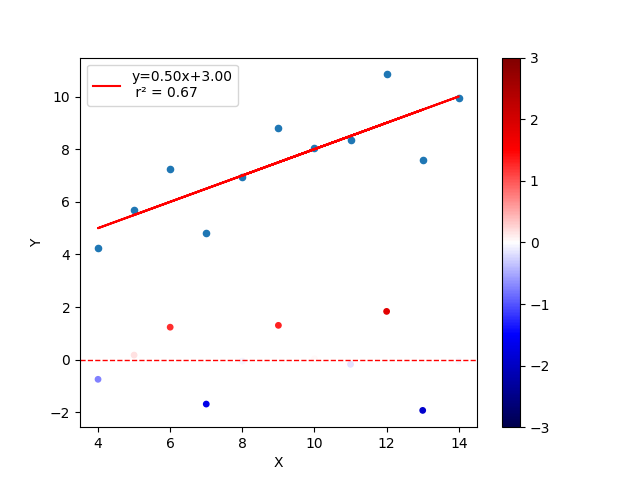
\includegraphics[width=0.45\linewidth]{dataset-res-1.png}}\qquad
\subfloat[Dataset II]{\label{fig:rII}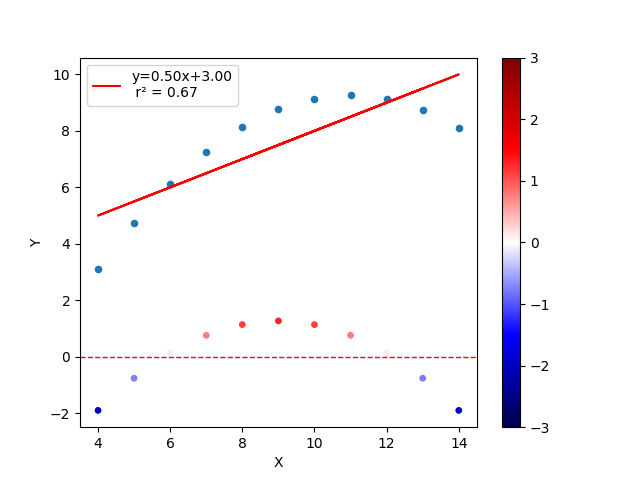
\includegraphics[width=0.45\linewidth]{dataset-res-2.png}}\\
\subfloat[Dataset III]{\label{fig:rIII}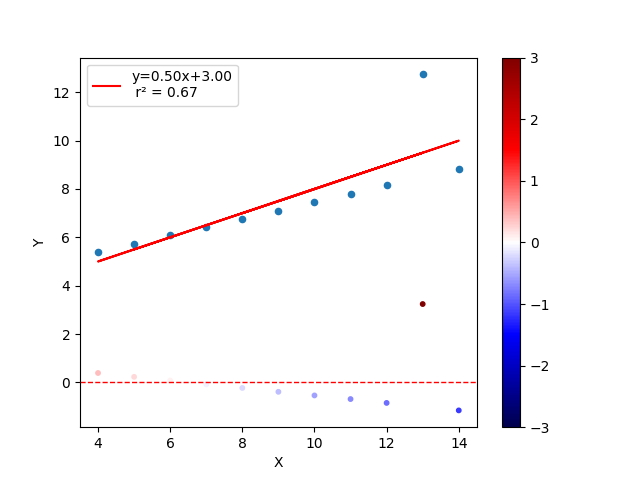
\includegraphics[width=0.45\textwidth]{dataset-res-3.png}}\qquad%
\subfloat[Dataset IV]{\label{fig:rIV}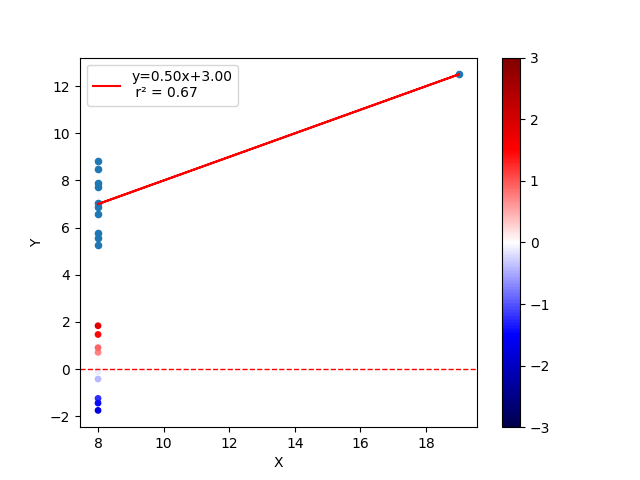
\includegraphics[width=0.45\textwidth]{dataset-res-4.png}}%
\caption{Residuals Plot of Datasets I-IV — X against Y with Lin. Reg.}
\label{fig:rplots}
\end{figure}

\end{document}